

\section{Results}


\subsection{Sample Problem}
The first test was on a problem with simple constraints and a pathological objective.
We let $f(x) = \epsilon x + (1-\epsilon)(y - \alpha x \sin(\gamma x))^2$ for a fixed constant $\epsilon$, and set the constraints to be
$x_2 \le ax_1$, $x_2 \ge -ax_1$ for a fixed constant $a$.

We summarize the number of function evaluations and iterations taken here:
\begin{center}
\begin{tabular}{ c c c c c c c c }
Shape & Search & Num. Segments & Basis & Iterations & Evaluations \\
\hline
                spherical &   anywhere &       &     linear & 159  &   202  &  470 &  630 \\
                spherical &   anywhere &       &  quadratic & 164  &   277  &  467 &  805 \\
                spherical &       none &       &     linear &  77* &   122* &  255 &  387 \\
                spherical &       none &       &  quadratic &  74  &   149  &  250 &  561 \\
                spherical &    segment &     1 &     linear &  74  &   116  &  224 &  413 \\
                spherical &    segment &     1 &  quadratic &  74  &   164  &  224 &  525 \\
                spherical &    segment &     2 &     linear & 164  &   223  &  313 &  503 \\
                spherical &    segment &     2 &  quadratic & 152  &   259  &  313 &  657 \\
  circumscribed ellipsoid &       none &       &     linear &  41  &    50  &   41 &   55 \\
  circumscribed ellipsoid &       none &       &  quadratic &  41  &   104  &   41 &  105 \\
                ellipsoid &   anywhere &       &     linear &  65  &   109  &   67 &  110 \\
                ellipsoid &   anywhere &       &  quadratic &  66  &   170  &   67 &  185 \\
%                ellipsoid &  anywhere* &       &  quadratic &  61  &   157  &   60 &  155 \\
                ellipsoid &       none &       &     linear &  53  &    65  &   50 &   52 \\
                ellipsoid &       none &       &  quadratic &  53  &    88  &   50 &   75 \\
                ellipsoid &    segment &     1 &     linear &  55  &    70  &   58 &   75 \\
                ellipsoid &    segment &     1 &  quadratic &  55  &    97  &   58 &  104 \\
                ellipsoid &    segment &     2 &     linear &  67  &   144  &   68 &  121 \\
                ellipsoid &    segment &     2 &  quadratic &  67  &   196  &   64 &  159 \\
               polyhedral &       none &       &     linear &  37  &    43  &   38 &   46 \\
               polyhedral &       none &       &  quadratic &  37  &    82  &   38 &   89 \\
         scaled ellipsoid &   anywhere &       &     linear &  66  &   103  &   67 &  104 \\
         scaled ellipsoid &   anywhere &       &  quadratic &  68  &   156  &   67 &  169 \\
         scaled ellipsoid &    segment &     1 &     linear &  44  &    65  &   45 &   67 \\
         scaled ellipsoid &    segment &     1 &  quadratic &  44  &    94  &   45 &   93 \\
         scaled ellipsoid &    segment &     2 &     linear &  67  &   125  &   68 &  122 \\
         scaled ellipsoid &    segment &     2 &  quadratic &  67  &   189  &   63 &  146 \\
                  simplex & max volume &       &     linear &  41  &    44  &   41 &   45 \\
                  simplex & max volume &       &  quadratic &  41  &    94  &   41 &   84 \\

%                spherical &   anywhere &       &     linear &   159 &   202 \\
%                spherical &   anywhere &       &  quadratic &   164 &   277 \\
%                spherical &       none &       &     linear &    77* &   122* \\
%                spherical &       none &       &  quadratic &    74 &   149 \\
%                spherical &    segment &     1 &     linear &    74 &   116 \\
%                spherical &    segment &     1 &  quadratic &    74 &   164 \\
%                spherical &    segment &     2 &     linear &   164 &   223 \\
%                spherical &    segment &     2 &  quadratic &   152 &   259 \\
%  circumscribed ellipsoid &       none &       &     linear &    41 &    50 \\
%  circumscribed ellipsoid &       none &       &  quadratic &    41 &   104 \\
%                ellipsoid &   anywhere &       &     linear &    65 &   109 \\
%                ellipsoid &   anywhere &       &  quadratic &    66 &   170 \\
%                ellipsoid &  anywhere* &       &  quadratic &    61 &   157 \\
%                ellipsoid &       none &       &     linear &    53 &    65 \\
%                ellipsoid &       none &       &  quadratic &    53 &    88 \\
%                ellipsoid &    segment &     1 &     linear &    55 &    70 \\
%                ellipsoid &    segment &     1 &  quadratic &    55 &    97 \\
%                ellipsoid &    segment &     2 &     linear &    67 &   144 \\
%                ellipsoid &    segment &     2 &  quadratic &    67 &   196 \\
%               polyhedral &       none &       &     linear &    37 &    43 \\
%               polyhedral &       none &       &  quadratic &    37 &    82 \\
%         scaled ellipsoid &   anywhere &       &     linear &    66 &   103 \\
%         scaled ellipsoid &   anywhere &       &  quadratic &    68 &   156 \\
%         scaled ellipsoid &    segment &     1 &     linear &    44 &    65 \\
%         scaled ellipsoid &    segment &     1 &  quadratic &    44 &    94 \\
%         scaled ellipsoid &    segment &     2 &     linear &    67 &   125 \\
%         scaled ellipsoid &    segment &     2 &  quadratic &    67 &   189 \\
%                  simplex & max volume &       &     linear &    41 &    44 \\
%                  simplex & max volume &       &  quadratic &    41 &    94 \\

\end{tabular}
\end{center}

*The spherical trust region with no search for the center did not converge.

In general, the linear models converge more quickly than quadratic models.
We see that the method with fewest iterations and function evaluations is the linear polyhedral shape.
This is likely due to the fact that the polyhedral shape is allowed to search the entire outer trust region.
This also explains why the circumscribed ellipse and maximum volume simplex also perform well.
%We also notices that with a simple heuristic we were able to improve the ellipse slightly from 170 to 157.
Also, the scaled ellipsoid performs comparably to the unscaled version.

\subsection{Schittkowksi Test Problems for Nonlinear Optimization}


We tested these algorithms on several problems from the Hot-Schittkowski problem set \cite{Schittkowski:1987:MTE:27135}, \cite{Hock1980}.
We selected the problems that have linear constraints: 21, 24, 25, 35, 36, 44, 45, 76, 224, 231, 232, 250, 251.

% 37 was left out because it proved to be difficult.

We summarize the results here.
\begin{tiny}

\begin{center}
\begin{tabular}{ c c c c c c c c c c }
Algorithm & Prob. & n & Message & N. It. & N. Eval. & Ret. Min. & Min. & Solution & Minimizer \\
\hline
  circumscribed ellipse   &   21  &  2  & converged  &   24  &   71  &  -99.960   &  -99.960   & [2.00,0.00] & [2.00,0.00] \\
         ellipse          &   21  &  2  & converged  &   36  &   96  &  -99.960   &  -99.960   & [2.00,0.00] & [2.00,0.00] \\
    ellipse everywhere    &   21  &  2  & converged  &   24  &   82  &  -99.960   &  -99.960   & [2.00,0.00] & [2.00,0.00] \\
    ellipse segment 1     &   21  &  2  & converged  &   24  &   84  &  -99.960   &  -99.960   & [2.00,0.00] & [2.00,0.00] \\
    ellipse segment 2     &   21  &  2  & converged  &   24  &   85  &  -99.960   &  -99.960   & [2.00,0.00] & [2.00,0.00] \\
        polyhedral        &   21  &  2  & converged  &   26  &   75  &  -99.960   &  -99.960   & [2.00,-0.00] & [2.00,0.00] \\
  circumscribed ellipse   &  224  &  2  &   failed   &   16  &   56  &  -304.000  &  -304.000  & [4.00,4.00] & [4.00,4.00] \\
         ellipse          &  224  &  2  & converged  &   32  &   97  &  -304.000  &  -304.000  & [4.00,4.00] & [4.00,4.00] \\
    ellipse everywhere    &  224  &  2  & converged  &   24  &   94  &  -303.774  &  -304.000  & [3.73,4.27] & [4.00,4.00] \\
    ellipse segment 1     &  224  &  2  & converged  &   24  &   91  &  -303.774  &  -304.000  & [3.73,4.27] & [4.00,4.00] \\
    ellipse segment 2     &  224  &  2  & converged  &   23  &   89  &  -303.774  &  -304.000  & [3.73,4.27] & [4.00,4.00] \\
        polyhedral        &  224  &  2  & converged  &   17  &   64  &  -304.000  &  -304.000  & [4.00,4.00] & [4.00,4.00] \\
  circumscribed ellipse   &  231  &  2  & converged  &   14  &   44  &   0.000    &   0.000    & [1.00,1.00] & [1.00,1.00] \\
         ellipse          &  231  &  2  & converged  &   99  &  193  &   0.000    &   0.000    & [1.00,1.00] & [1.00,1.00] \\
    ellipse everywhere    &  231  &  2  & converged  &  181  &  336  &   0.000    &   0.000    & [1.00,1.00] & [1.00,1.00] \\
    ellipse segment 1     &  231  &  2  & converged  &   78  &  162  &   0.000    &   0.000    & [1.00,1.00] & [1.00,1.00] \\
    ellipse segment 2     &  231  &  2  & converged  &  173  &  321  &   0.000    &   0.000    & [1.00,1.00] & [1.00,1.00] \\
        polyhedral        &  231  &  2  & converged  &   95  &  193  &   0.000    &   0.000    & [1.00,1.00] & [1.00,1.00] \\
  circumscribed ellipse   &  232  &  2  &   failed   &   15  &   35  &   -1.000   &   -1.000   & [3.00,1.73] & [3.00,1.73] \\
         ellipse          &  232  &  2  & converged  &   34  &   91  &   -1.000   &   -1.000   & [3.00,1.73] & [3.00,1.73] \\
    ellipse everywhere    &  232  &  2  & converged  &   41  &  102  &   -1.000   &   -1.000   & [3.00,1.73] & [3.00,1.73] \\
    ellipse segment 1     &  232  &  2  & converged  &   34  &   91  &   -1.000   &   -1.000   & [3.00,1.73] & [3.00,1.73] \\
    ellipse segment 2     &  232  &  2  & converged  &   35  &   95  &   -1.000   &   -1.000   & [3.00,1.73] & [3.00,1.73] \\
        polyhedral        &  232  &  2  & converged  &   15  &   47  &   -1.000   &   -1.000   & [3.00,1.73] & [3.00,1.73] \\
  circumscribed ellipse   &   24  &  2  &   failed   &   15  &   35  &   -1.000   &   -1.000   & [3.00,1.73] & [3.00,1.73] \\
         ellipse          &   24  &  2  & converged  &   34  &   90  &   -1.000   &   -1.000   & [3.00,1.73] & [3.00,1.73] \\
    ellipse everywhere    &   24  &  2  & converged  &   41  &  104  &   -1.000   &   -1.000   & [3.00,1.73] & [3.00,1.73] \\
    ellipse segment 1     &   24  &  2  & converged  &   34  &   91  &   -1.000   &   -1.000   & [3.00,1.73] & [3.00,1.73] \\
    ellipse segment 2     &   24  &  2  & converged  &   35  &   95  &   -1.000   &   -1.000   & [3.00,1.73] & [3.00,1.73] \\
        polyhedral        &   24  &  2  & converged  &   15  &   47  &   -1.000   &   -1.000   & [3.00,1.73] & [3.00,1.73] \\
  circumscribed ellipse   &  250  &  3  &   failed   &   24  &  103  & -3300.000  & -3300.000  & [20.00,11.00,15.00] & [20.00,11.00,15.00] \\
         ellipse          &  250  &  3  & converged  &   53  &  207  & -3300.000  & -3300.000  & [20.00,11.00,15.00] & [20.00,11.00,15.00] \\
    ellipse everywhere    &  250  &  3  &   failed   &   48  &  103  & -3298.196  & -3300.000  & [19.99,10.99,15.02] & [20.00,11.00,15.00] \\
    ellipse segment 1     &  250  &  3  &   failed   &   53  &  112  & -3299.243  & -3300.000  & [19.99,11.00,15.01] & [20.00,11.00,15.00] \\
    ellipse segment 2     &  250  &  3  &   failed   &   54  &  112  & -3299.082  & -3300.000  & [19.99,11.00,15.01] & [20.00,11.00,15.00] \\
    ellipse segment 3     &  250  &  3  &   failed   &   56  &  116  & -3299.504  & -3300.000  & [19.99,11.00,15.00] & [20.00,11.00,15.00] \\
        polyhedral        &  250  &  3  & converged  &   26  &  113  & -3300.000  & -3300.000  & [20.00,11.00,15.00] & [20.00,11.00,15.00] \\
  circumscribed ellipse   &  251  &  3  &   failed   &   20  &   86  & -3456.000  & -3456.000  & [24.00,12.00,12.00] & [24.00,12.00,12.00] \\
         ellipse          &  251  &  3  &   failed   &   10  &   53  & -3454.018  & -3456.000  & [23.55,12.06,12.16] & [24.00,12.00,12.00] \\
    ellipse everywhere    &  251  &  3  &   failed   &   6   &   17  & -3209.710  & -3456.000  & [22.82,13.03,10.79] & [24.00,12.00,12.00] \\
    ellipse segment 1     &  251  &  3  &   failed   &   4   &   13  & -1698.807  & -3456.000  & [21.71,9.21,8.50] & [24.00,12.00,12.00] \\
    ellipse segment 2     &  251  &  3  &   failed   &   6   &   17  & -3210.341  & -3456.000  & [21.49,11.46,13.04] & [24.00,12.00,12.00] \\
    ellipse segment 3     &  251  &  3  &   failed   &   14  &   64  & -3449.803  & -3456.000  & [22.84,12.29,12.29] & [24.00,12.00,12.00] \\
        polyhedral        &  251  &  3  & converged  &   22  &  124  & -3456.000  & -3456.000  & [24.00,12.00,12.00] & [24.00,12.00,12.00] \\
  circumscribed ellipse   &   25  &  3  & converged  &  760  &  1472 &   0.000    &   0.000    & [52.92,24.90,1.52] & [50.00,25.00,1.50] \\
    ellipse everywhere    &   25  &  3  &   failed   &   1   &   1   &   32.835   &   0.000    & [100.00,12.50,3.00] & [50.00,25.00,1.50] \\
    ellipse segment 1     &   25  &  3  &   failed   &   1   &   1   &   32.835   &   0.000    & [100.00,12.50,3.00] & [50.00,25.00,1.50] \\
    ellipse segment 2     &   25  &  3  &   failed   &   1   &   1   &   32.835   &   0.000    & [100.00,12.50,3.00] & [50.00,25.00,1.50] \\
    ellipse segment 3     &   25  &  3  &   failed   &   1   &   1   &   32.835   &   0.000    & [100.00,12.50,3.00] & [50.00,25.00,1.50] \\
        polyhedral        &   25  &  3  & converged  &  1793 &  3396 &   0.000    &   0.000    & [50.94,24.97,1.51] & [50.00,25.00,1.50] \\
  circumscribed ellipse   &   35  &  3  &   failed   &  781  &  1028 &   0.111    &   0.111    & [1.33,0.78,0.44] & [1.33,0.78,0.44] \\
         ellipse          &   35  &  3  & converged  &   28  &  122  &   0.111    &   0.111    & [1.33,0.78,0.44] & [1.33,0.78,0.44] \\
    ellipse everywhere    &   35  &  3  &   failed   &   24  &   82  &   0.113    &   0.111    & [1.36,0.79,0.42] & [1.33,0.78,0.44] \\
    ellipse segment 1     &   35  &  3  &   failed   &   16  &   76  &   0.112    &   0.111    & [1.31,0.79,0.45] & [1.33,0.78,0.44] \\
    ellipse segment 2     &   35  &  3  &   failed   &   16  &   75  &   0.112    &   0.111    & [1.31,0.79,0.45] & [1.33,0.78,0.44] \\
    ellipse segment 3     &   35  &  3  &   failed   &   16  &   77  &   0.112    &   0.111    & [1.31,0.79,0.45] & [1.33,0.78,0.44] \\
        polyhedral        &   35  &  3  & converged  &   14  &  112  &   0.111    &   0.111    & [1.33,0.78,0.44] & [1.33,0.78,0.44] \\
  circumscribed ellipse   &   36  &  3  &   failed   &   19  &   81  & -3300.000  & -3300.000  & [20.00,11.00,15.00] & [20.00,11.00,15.00] \\
         ellipse          &   36  &  3  & converged  &   53  &  202  & -3300.000  & -3300.000  & [20.00,11.00,15.00] & [20.00,11.00,15.00] \\
    ellipse everywhere    &   36  &  3  &   failed   &   63  &  135  & -3299.808  & -3300.000  & [20.00,11.00,15.00] & [20.00,11.00,15.00] \\
    ellipse segment 1     &   36  &  3  &   failed   &   64  &  140  & -3299.951  & -3300.000  & [20.00,11.00,15.00] & [20.00,11.00,15.00] \\
    ellipse segment 2     &   36  &  3  &   failed   &   64  &  133  & -3299.918  & -3300.000  & [20.00,11.00,15.00] & [20.00,11.00,15.00] \\
    ellipse segment 3     &   36  &  3  &   failed   &   65  &  137  & -3299.870  & -3300.000  & [20.00,11.00,15.00] & [20.00,11.00,15.00] \\
        polyhedral        &   36  &  3  & converged  &   22  &  108  & -3300.000  & -3300.000  & [20.00,11.00,15.00] & [20.00,11.00,15.00] \\
  circumscribed ellipse   &   37  &  3  &   failed   &   27  &   98  & -3456.000  & -3456.000  & [24.00,12.00,12.00] & [24.00,12.00,12.00] \\
         ellipse          &   37  &  3  &   failed   &   15  &   65  & -3455.761  & -3456.000  & [23.94,12.01,12.02] & [24.00,12.00,12.00] \\
    ellipse everywhere    &   37  &  3  &   failed   &   36  &   88  & -3406.653  & -3456.000  & [27.34,10.93,11.40] & [24.00,12.00,12.00] \\
    ellipse segment 1     &   37  &  3  &   failed   &   30  &   82  & -3421.619  & -3456.000  & [21.29,12.62,12.73] & [24.00,12.00,12.00] \\
    ellipse segment 2     &   37  &  3  &   failed   &   36  &   85  & -3415.110  & -3456.000  & [21.05,12.70,12.78] & [24.00,12.00,12.00] \\
    ellipse segment 3     &   37  &  3  &   failed   &   28  &   75  & -3421.157  & -3456.000  & [21.31,12.55,12.79] & [24.00,12.00,12.00] \\
        polyhedral        &   37  &  3  & converged  &   28  &  139  & -3456.000  & -3456.000  & [24.00,12.00,12.00] & [24.00,12.00,12.00] \\
  circumscribed ellipse   &   44  &  4  &   failed   &   17  &  124  &  -13.000   &  -15.000   & [3.00,-0.00,4.00,0.00] & [0.00,3.00,0.00,4.00] \\
         ellipse          &   44  &  4  & converged  &   50  &  298  &  -15.000   &  -15.000   & [0.00,3.00,-0.00,4.00] & [0.00,3.00,0.00,4.00] \\
    ellipse everywhere    &   44  &  4  & converged  &  110  &  416  &  -15.000   &  -15.000   & [0.00,3.00,0.00,4.00] & [0.00,3.00,0.00,4.00] \\
    ellipse segment 1     &   44  &  4  & converged  &   50  &  262  &  -15.000   &  -15.000   & [-0.00,3.00,0.00,4.00] & [0.00,3.00,0.00,4.00] \\
    ellipse segment 2     &   44  &  4  & converged  &   71  &  304  &  -15.000   &  -15.000   & [-0.00,3.00,0.00,4.00] & [0.00,3.00,0.00,4.00] \\
    ellipse segment 3     &   44  &  4  &   failed   &   7   &   32  &  -10.672   &  -15.000   & [-0.00,2.55,0.36,3.41] & [0.00,3.00,0.00,4.00] \\
    ellipse segment 4     &   44  &  4  &   failed   &   1   &   1   &   -1.338   &  -15.000   & [1.44,0.98,1.80,1.80] & [0.00,3.00,0.00,4.00] \\
        polyhedral        &   44  &  4  & converged  &   15  &  134  &  -13.000   &  -15.000   & [3.00,-0.00,4.00,-0.00] & [0.00,3.00,0.00,4.00] \\
  circumscribed ellipse   &   45  &  5  &   failed   &   21  &  190  &   1.000    &   1.000    & [1.00,2.00,3.00,4.00,5.00] & [1.00,2.00,3.00,4.00,5.00] \\
         ellipse          &   45  &  5  & converged  &   51  &  405  &   1.000    &   1.000    & [1.00,2.00,3.00,4.00,5.00] & [1.00,2.00,3.00,4.00,5.00] \\
    ellipse everywhere    &   45  &  5  & converged  &  414  &  1121 &   1.000    &   1.000    & [1.00,2.00,3.00,4.00,5.00] & [1.00,2.00,3.00,4.00,5.00] \\
    ellipse segment 1     &   45  &  5  & converged  &   63  &  374  &   1.000    &   1.000    & [1.00,2.00,3.00,4.00,5.00] & [1.00,2.00,3.00,4.00,5.00] \\
    ellipse segment 2     &   45  &  5  & converged  &   82  &  404  &   1.000    &   1.000    & [1.00,2.00,3.00,4.00,5.00] & [1.00,2.00,3.00,4.00,5.00] \\
    ellipse segment 3     &   45  &  5  & converged  &  104  &  453  &   1.000    &   1.000    & [1.00,2.00,3.00,4.00,5.00] & [1.00,2.00,3.00,4.00,5.00] \\
    ellipse segment 4     &   45  &  5  & converged  &  130  &  497  &   1.000    &   1.000    & [1.00,2.00,3.00,4.00,5.00] & [1.00,2.00,3.00,4.00,5.00] \\
    ellipse segment 5     &   45  &  5  & converged  &  158  &  478  &   1.000    &   1.000    & [1.00,2.00,3.00,4.00,5.00] & [1.00,2.00,3.00,4.00,5.00] \\
        polyhedral        &   45  &  5  & converged  &   22  &  269  &   1.000    &   1.000    & [1.00,2.00,3.00,4.00,5.00] & [1.00,2.00,3.00,4.00,5.00] \\
  circumscribed ellipse   &   76  &  4  &   failed   &   15  &  111  &   -4.682   &   -4.682   & [0.27,2.09,-0.00,0.55] & [0.27,2.09,-0.00,0.55] \\
         ellipse          &   76  &  4  &   failed   &   17  &  137  &   -4.682   &   -4.682   & [0.27,2.09,0.00,0.54] & [0.27,2.09,-0.00,0.55] \\
    ellipse everywhere    &   76  &  4  &   failed   &   25  &  106  &   -4.604   &   -4.682   & [0.45,1.89,-0.00,0.77] & [0.27,2.09,-0.00,0.55] \\
    ellipse segment 1     &   76  &  4  &   failed   &   17  &  111  &   -4.682   &   -4.682   & [0.27,2.09,-0.00,0.54] & [0.27,2.09,-0.00,0.55] \\
    ellipse segment 2     &   76  &  4  &   failed   &   24  &  105  &   -4.680   &   -4.682   & [0.31,2.08,0.00,0.52] & [0.27,2.09,-0.00,0.55] \\
    ellipse segment 3     &   76  &  4  &   failed   &   25  &  106  &   -4.677   &   -4.682   & [0.34,2.07,0.00,0.51] & [0.27,2.09,-0.00,0.55] \\
    ellipse segment 4     &   76  &  4  &   failed   &   23  &  107  &   -4.674   &   -4.682   & [0.34,2.03,-0.00,0.60] & [0.27,2.09,-0.00,0.55] \\
        polyhedral        &   76  &  4  & converged  &   15  &  169  &   -4.682   &   -4.682   & [0.27,2.09,-0.00,0.55] & [0.27,2.09,-0.00,0.55]
\end{tabular}
\end{center}


\end{tiny}

In order to better evaluate the algorithms on the problems across in this test set, we use a performance profile developed in \cite{More:2009:BDO:1654367.1654371}.
Given a set of Solvers $\mathcal S$ that solved a set of problems $\mathcal P$ with the number of evaluations of solver $s$ on problem $p$ being $N(s, p)$, the performance ratio is defined to be $r(s, p) = \frac{N(s, p)}{\min_{s \in \mathcal S} N(s, p)}$.
If the algorithm does not complete, then the number of evaluations is set to $\infty$.
The performance profile of a solver $s$ and parameter $\alpha \in [0, \infty)$ is then the number of problems for which the performance ratio is less than or equal to $\alpha$: 

\begin{align}
\rho(s, \alpha) = \frac 1 {\|\mathcal P \|} \|p \in \mathcal P | r(s, p) \le \alpha\|.
\end{align}

The $y$ axis of a performance plot is the performance profile, and the $x$ axis is the parameter $\alpha$.
Note that algorithms with high performance profiles for small values of $alpha$ solved a large number of problems the most with the fewest evaluations, while algorithms that eventually reach high performance profiles with larger values of $\alpha$ solve a large set of problems.
The performance profile for the Hot-Schittkowski problem set is give in figure \cref{performance_profile}.


\begin{figure}[h]
    \centering
    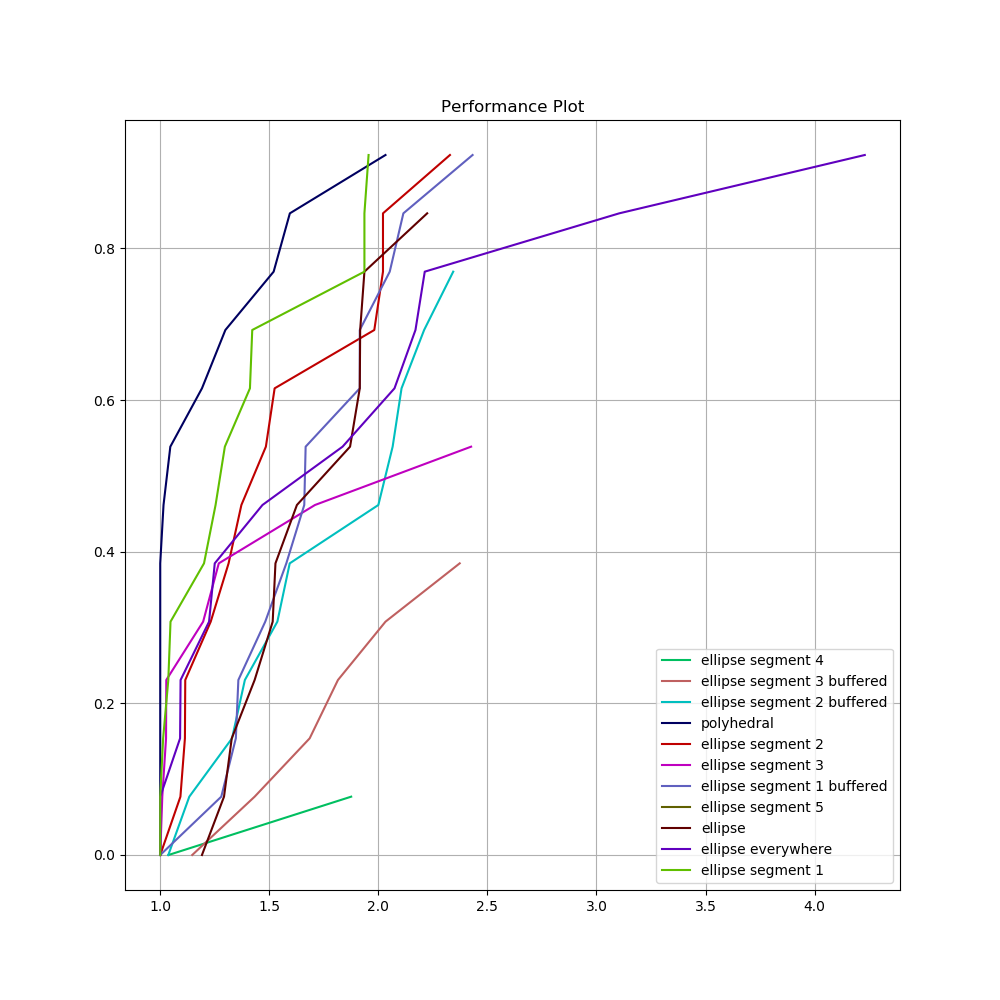
\includegraphics[scale=0.4]{images/performance_profile_plot.png}
    \caption{Performance profile}
    \label{performance_profile}
\end{figure}



The line segment search with 5 segments does not solve many problems, this is because several of the problems have dimension less than $5$, so that it was not even ran on these.
Notice that the polyhedral search does very well.
We conjecture that this may not hold with modelled, nonlinear constraints.




\subsection{Summary}
We still experienced a problem with iterates coming too close to the boundary of the feasible region.
Another way of dealing with this is to shift the constraints closer to the current iterate.
Namely, we introduce a parameter $\upsilon$ to determine how far to scale the constraints.
Then, within the trust region subproblem, we add constraints of $Ax \le b\upsilon + (1-\upsilon) A\iteratek$.
Before doing this, the rows of $A$ are normalized.
This produces the buffered segment searches withing the results.

%Add another column for $a$.
%Want to average over multiple starting points.
%Include a runtime for each (will hurt ellipses).
